\documentclass[%
aip,
jmp,
reprint,
floatfix,
nofootinbib
]{revtex4-1}

\usepackage{graphicx}% Include figure files
\usepackage{dcolumn}% Align table columns on decimal point
\usepackage{bm}% bold math
\usepackage{float}
\usepackage{siunitx}
\usepackage{hyperref}
\usepackage{listings}
\usepackage[english]{babel}
\usepackage[utf8]{inputenc}
\usepackage[]{natbib}
\bibliographystyle{plainnat}
\usepackage{ gensymb }
%\usepackage[mathlines]{lineno}% Enable numbering of text and display math
%\linenumbers\relax % Commence numbering lines
\usepackage{color}
\usepackage{subcaption}

\definecolor{dkgreen}{rgb}{0,0.6,0}
\definecolor{gray}{rgb}{0.5,0.5,0.5}
\definecolor{mauve}{rgb}{0.58,0,0.82}

\lstset{
	frame=single, 
	language=Python, 
	columns=flexible,
	basicstyle={\footnotesize\ttfamily},
	keywordstyle=\color{blue},
	commentstyle=\color{dkgreen},
	stringstyle=\color{red},
	title=\lstname
}


\renewcommand{\arraystretch}{1.3} % Changes the height of tables
\DeclareSIUnit\year{yr}
\DeclareSIUnit\parsec{pc}



\begin{document}

	\title[WCS Coordinates with M29]{Using the WCS Coordinate System with M29}

	\author{Lucas, Miles}
	\author{Brandon, John}
	\affiliation{Iowa State University Department of Physics and Astronomy}

	\date{\today}


% Write here a short abstract (1 paragraph) describing what you achieved in this lab.

	\begin{abstract}
	In this lab we achieved in applying a coordinate system to images of open galactic cluster M29. By using a reference DSS image, we used Koords, SAO ds9, and AstroImageJ to calculate, align, and apply the WCS coordinate system. From this we calculated the pixel scale to be \SI{1.165\pm.027}{\arcsecond\per p} for each axis. We also matched 16 stars to the Tycho-2 catalog. We composed an RGB image using our B, V, and I filter images but it was inaccurate due to inconsistencies in the sharpness of the images.

	\end{abstract}

	\maketitle
%________________________________________________________________________

%	Write here a summary of the goals of this lab. Be brief – do not exceed the end of the first page.

	\section{Introduction}

	The goals of this lab were to apply WCS coordinates to FITS images of M29 and then compose and RGB image using the B, V, and I filtered photos aligned with the coordinate system. M29 is an open galactic cluster about \SI{1.1}{\kilo\parsec} away from our system and approximately \SI{10}{\mega\year} old. It contains at least 50 stars and is located about \ang{1.7} from Sadr\citep{labman}.

	The benefit of having a coordinate system applied to the image allows much more research flexibility. With a known position it is possible to automatically find stars from a catalog. It is also useful to be able to align and rotate images to show celestial North and East correctly. It is also great for stacking photos that have all been aligned.
	
	RGB images are great for visually seeing the color of stars. This is great for categorizing stars according to their spectral type. Generally, the hotter the star, the bluer it is visually.
	
%________________________________________________________________________

%	Describe your telescope and camera setup. For the first lab you should describe the setup in more details. Subsequent labs can refer to the procedure described in the first lab, and focus more on the data acquisition itself. Important details to write include: which stars have been observed, which filters were used (BVI), what exposure times and what calibration procedures have been followed (e.g., dark frames acquisition, photometric standards observed, etc.). Mention also the observing conditions (weather, moon presence, temperature, etc.). You should include the observing log appendix A (a table or a scan of a hardcopy). This section can be as long as necessary, but you should strive for brevity (you can refer to the lab guide to avoid repeating all steps, but make sure you explain anything you did differently, problems encountered, etc.). Use tables to summarize information clearly.

	\section{Data Acquisition and Setup}
	Observations were made on \date{06 September 2017} at the Zaffarano Hall observation deck in Ames, Iowa (\ang{-93.64734}, \ang{42.02996}, \SI{342}{\meter}). The night was mostly clear and the ambient temperature was around \SI{12}{\degreeCelsius}. The moon was waning that night and had little to no effect on our sight. Observations were made using a Meade 8" reflector telescope with an SBIG ST-402ME CCD camera with internal V, B, and I filters. 
	
	Setting up the telescope was the same as previous observations made with the 8" Meade telescope at Zaffarano Hall. We took \num{15} images of M29, five in each photometric filter from B, V, and I. We used a \SI{20}{\second} exposure for all the images in addition to five dark frames. Getting sharp images was difficult in our observations due to the long exposure time. We needed such long times due to the vaintness of the stars in the cluster, but ambient vibrations on the deck as well as the drift of the equatorial mount caused blurriness and sometimes streaking.

%________________________________________________________________________

%Describe what you did to analyze the data. For the first lab this section will be minimal. For subsequent labs you should describe in detail the steps you did to analyze the data.  If applicable you can attach the code you used to analyze the data in Appendix B (either a log of your IDL section, or the code of any scripts you wrote). You can also attach screenshots of your computer session if it helps your discussion. Include tables of raw data in this section. The goal of this section is to describe unambiguously what you did to derive your final images and measured quantities from the raw data. Again be brief but complete (use as much space as you need).
	\section{Data Analysis}
	
	To process each image, we used AstroIamgeJ's data reduction facility to create the median dark frame and subtract it from each image. For more information, see our lab report regarding Albireo and its analysis. 
	
	\subsection{Calculating and Applying Coordinate System}
	To apply our coordinate system, we used the program Koords, which calculates the orientation of an image and then maps the coordinate system onto it using a reference image with the coordinates already applied. Koords accomplishes this by pairing the objects in both the reference and target images for at least three objects and then triangulating the orientation. The reference image we used is shown in \autoref{fig:dss}.
	
	Examples of our corrected images are in \autoref{fig:b}, \autoref{fig:v}, and \autoref{fig:i}. Koords automatically rewrites the FITS headers to describe their alignment correction factors and the pixel scales with keywords `CDELT1' and `CDELT2'. \autoref{lst:imscale} parses this information from every corrected image and reports the 95\% confidence interval for the pixel scale in the x and y directions of the image. 
	
	\subsection{Catalog Analysis}
	Using SAO ds9 we analyzed the image for its stars using the Tycho-2 catalog. In order to get the spectral class for these stars, we had to do a similar analysis using the SIMBAD catalog and match those results with the Tycho-2 results.
	
	\subsection{Alignment and RGB Composition}
	Lastly, we stacked our sharpest B, V, and I images to compose an RGB photo of M29. To align our images we used AstroImageJ which aligned all of our WCS corrected images and saved them as new files. Of these we choose our best from each filter and loaded them into Adobe Photoshop CC. NASA has an automation script \citep{fits}. for preparing the filter layers of our image. Although we could have done this in ds9 or AstroImageJ, we felt like we had the most control and ease of use with Photoshop. 
	
	The method in which Photoshop composes the image is by applying adjustments to each layer in the file. The adjustment layers made were hue, curve, and levels. Hue adjustment gave the layers their red, green, or blue tone. We used the B image for our blue layer, the V image for our green layer, and the I image for our red layer. The curve adjustment is similar to applying a logorithmic or arcsine scale but instead allows adjusting the curve by grabbing and stretching it. We did not adjust this layer, which left us using a linear scale. The levels layer is the same as the scale adjustment in ds9 or AIJ. For each layer we played with the levels until we achieved fairly white stars and a fairly black background.
	
	

	
%________________________________________________________________________

%	Describe in detail the results you obtained from the quantitative analysis of your data, as explained in the lab guide.
	\section{Results}


	 Our 95\% confidence interval for the image scale in the x-direction (axis 1) was \SI{1.165\pm.027}{\arcsecond\per p} and \SI{1.165\pm.027}{\arcsecond\per p} in the y-direction (axis 2). The map of the results of the Tycho-2 catalog analysis are in \autoref{fig:map} and their corresponding information is in \autoref{table:tycho}. Note that we had to remove some entries for the Tycho-2 analysis because they appeared physically outside of our image. The aligned B, V, and I images are shown in \autoref{fig:b}, \autoref{fig:v}, and \autoref{fig:i}. Our RGB composed image is in \autoref{fig:rgb}. 

	
	

%________________________________________________________________________

%	Add here anything else you want to say, and summarize your results. This section should be very brief, not more than a couple of paragraphs
	\section{Conclusions}
	
	In our report on Albireo we calculated the pixel scale using the angular separation of the stars and received \SI{1.0072\pm.0091}{\arcsecond\per p}. That is similar to our result, with a difference of 15.7\%. We conclude the differences can be due to uncertainty in angular separation of the Albireo, the sometimes inconsistent Koords calculations, and the few blurry or streaky images still used in this calculation. We noted that the pixel scale was the same for each axis, which makes sense, because each pixel covers an equal distance in each direction.	
	
	Looking through the Tycho-2 catalog, we felt confident in the accuracy of the calculations, although it was mildly inefficient to have to use both the Tycho-2 and SIMBAD analysis tools to get all the information we wanted. Stepping forward, comparing the spectral type to the RGB image was not fruitful. The sharpest I filter image we have is blurrier than the other two layers, which causes an awkward lensing around the bright stars. This could also be an issue with differences in saturation for each filter because we used the same exposure time. On \autoref{fig:map} the brightest stars are often low B class stars, though they appear yellow-white in our image, which ought to correspond to a F to G type star. 
	
	We also wanted to note some difficulties we had with the Koords program. Not only is it slow, cumbersome, and inefficient for large sequences, but it also is prone to random segmentation errors. This was very frustrating for us, even going through our 15 science images.

%________________________________________________________________________

	\section*{Acknowledgments}

	Thank you to Dr. Charles Kerton and Brandon Marshall for their guidance and assistance in this work.
	\medskip
	\bibliography{refs}


%________________________________________________________________________

	\onecolumngrid
	\appendix
	\section{Observation Log}

	\begin{table}[H]
		\centering
		\caption{Observed 06 September 2017 by Miles Lucas and John Brandon}
\begin{tabular}{clclcccl}
	\hline
	Time  & File                   & N Frames & Object                                     & Filter &     Exposure     &       Camera Temp.        & Notes       \\ \hline\hline
	21:39 & M39\_2\_V\_13s\_       &    5     & M39 Objects x1, x4, x7, and x9; stars E, D &   V    & \SI{13}{\second} & \SI{5.33}{\degreeCelsius} &             \\
	21:41 & M39\_2\_V\_13s\_dark\_ &    5     & M39 Objects x1, x4, x7, and x9; stars E, D &   V    & \SI{13}{\second} & \SI{5.33}{\degreeCelsius} & Dark frames \\
	21:43 & M39\_2\_B\_13s\_       &    5     & M39 Objects x1, x4, x7, and x9; stars E, D &   B    & \SI{13}{\second} & \SI{5.33}{\degreeCelsius} &             \\ \hline
\end{tabular}

		\label{table:log}
	\end{table}	

	\section{Images and Tables} 
	
	\begin{figure}[H]
		\centering
		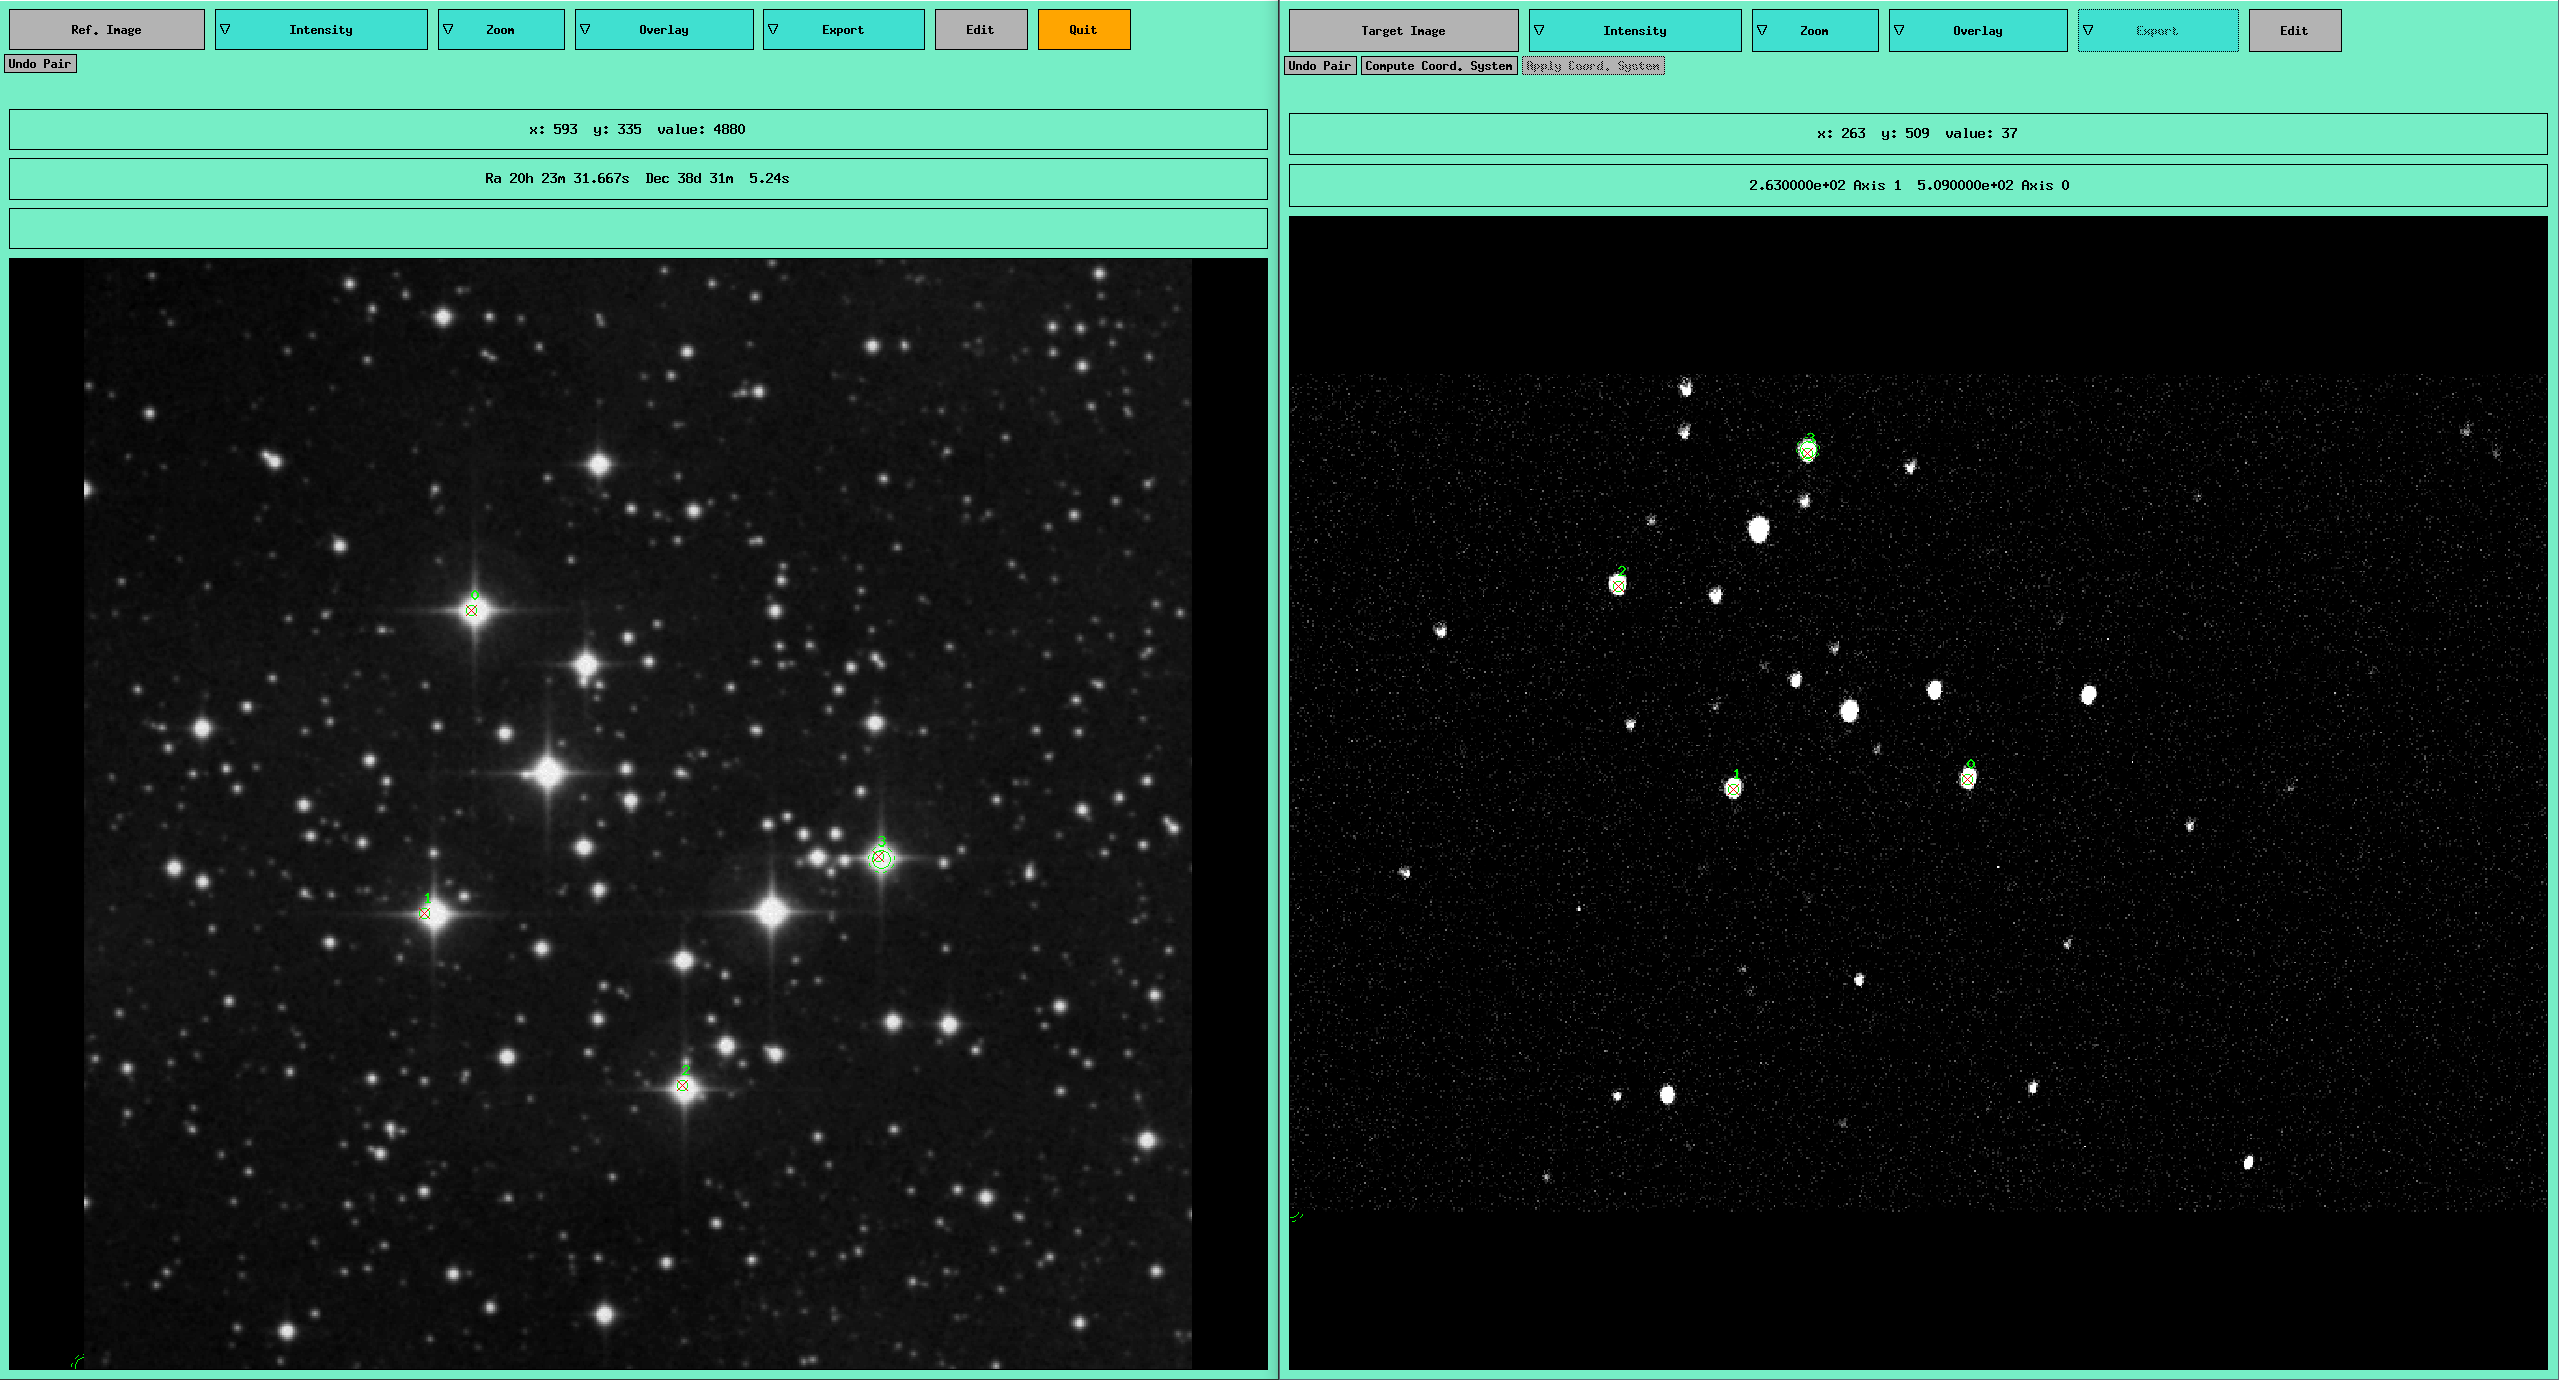
\includegraphics[width=.8\textwidth]{figs/koords.png}
		\caption{Using Koords to calculate and apply coordinate system to our photos. The pairs shown in this image were used in every image for calculations.}
		\label{fig:koords}
	\end{figure}
	
	\begin{figure}[H]
		\centering
		\begin{subfigure}[t]{.4\textwidth}
			\centering
			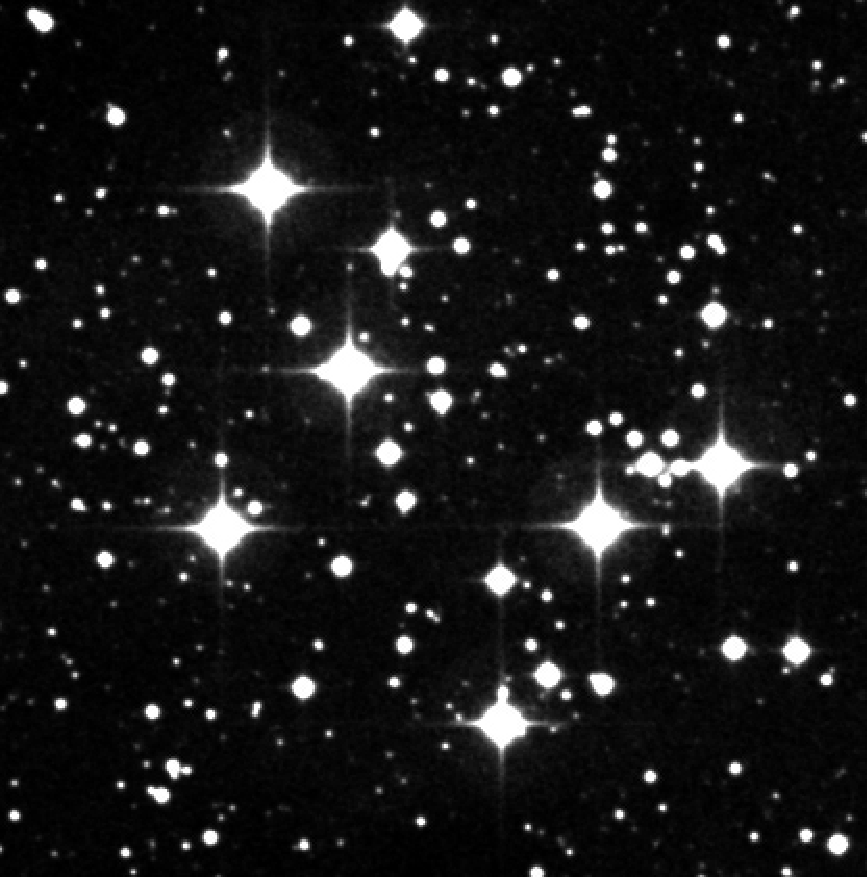
\includegraphics[width=\linewidth]{figs/dss.pdf}
			\caption{DSS POSSII image of M29}
			\label{fig:dss}
		\end{subfigure}
		\qquad
		\begin{subfigure}[t]{.4\textwidth}
			\centering
			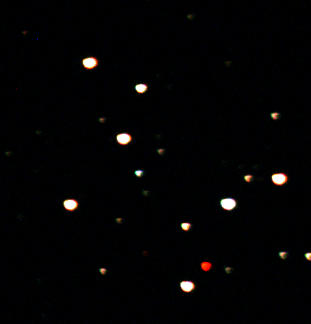
\includegraphics[width=\linewidth]{figs/rgb.pdf}
			\caption{RGB composed image of M29 from our B, V, and I images cropped to the seven brightest and most recognizable stars}
			\label{fig:rgb}
		\end{subfigure}
	\end{figure}
	
	
	\begin{figure}[H]
		\centering
		\begin{subfigure}[]{0.3\textwidth}
			\centering
			\includegraphics[width=\linewidth]{figs/b.pdf}
			\caption{Photometric B}
			\label{fig:b}
		\end{subfigure}
		\begin{subfigure}[]{0.3\textwidth}
			\centering
			\includegraphics[width=\linewidth]{figs/v.pdf}
			\caption{Photometric V}
			\label{fig:v}
		\end{subfigure}
		\begin{subfigure}[]{0.3\textwidth}
			\centering
			\includegraphics[width=\linewidth]{figs/i.pdf}
			\caption{Photometric I}
			\label{fig:i}
		\end{subfigure}
		\caption{WCS aligned images with celestial North and East oriented straight up and left on the image}
	\end{figure}

	\begin{figure}[H]
		\centering
		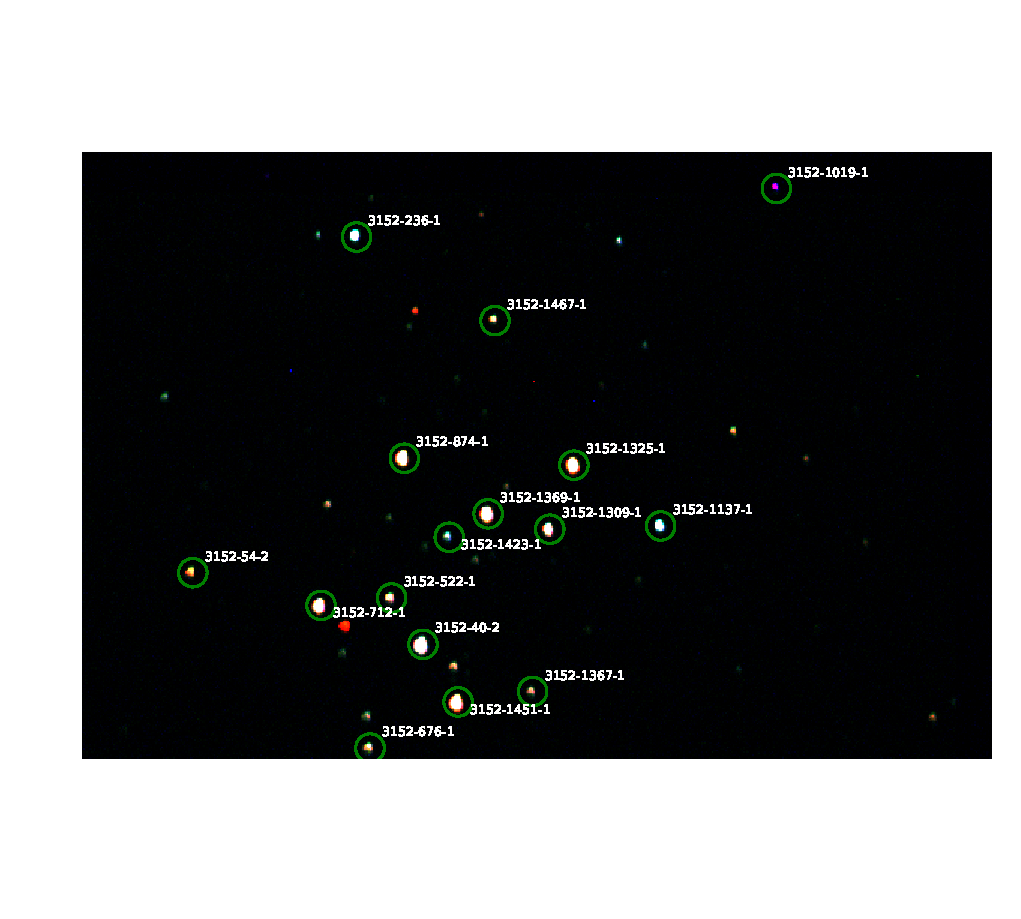
\includegraphics[width=\textwidth]{figs/map.pdf}
		\caption{The map of the Tycho-2 stars superimposed on our RGB image\protect\footnotemark}
		\label{fig:map}
	\end{figure}
	\footnotetext{This image was made using python sourced in the Jupyter Notebook from \autoref{sec:scripts}.}

	\begin{table}[H]
		\centering
		\caption{Information from the Tycho-2 and SIMBAD analysis of our WCS images}
\begin{tabular}{lllllllllllll}
	\hline\hline
	\_RAJ2000  & \_DEJ2000 & TYC1 & TYC2 & TYC3 & pmRA  & pmDE  & BTmag  & VTmag  & HIP    & RA(ICRS)    & DE(ICRS)    & SP Type    \\ \hline
	305.962521 & 38.49286  & 3152 & 40   & 1    & -13.3 & -11   & 9.113  & 8.645  & 100586 & 305.96256   & 38.49288528 & F0III      \\
	305.994691 & 38.432574 & 3152 & 54   & 1    & -0.9  & -5.5  & 12.964 & 11.652 &        & 305.9946933 & 38.43258639 & B1-1.5V    \\
	306.105109 & 38.485246 & 3152 & 236  & 1    & -1.4  & -5.2  & 10.293 & 10.181 &        & 306.1051136 & 38.48525833 & A2         \\
	305.979509 & 38.485578 & 3152 & 522  & 1    & -5.8  & -7.3  & 11.823 & 11.503 &        & 305.9795258 & 38.485595   & B2V        \\
	305.928488 & 38.475918 & 3152 & 676  & 1    & -2.8  & -20.3 & 12.128 & 12.094 &        & 305.9284961 & 38.475965   & B2V        \\
	305.979257 & 38.466345 & 3152 & 712  & 1    & -5.2  & -5.6  & 10.18  & 9.482  & 100600 & 305.9792722 & 38.4663575  & O9.7III(n) \\
	306.027282 & 38.492559 & 3152 & 874  & 1    & -2.8  & -4.4  & 9.923  & 9.108  & 100612 & 306.0272897 & 38.49256861 & B0.2III    \\
	306.108385 & 38.599753 & 3152 & 1019 & 1    & -3.4  & 3.6   & 11.923 & 11.358 &        & 306.1083947 & 38.59974472 &            \\
	305.995611 & 38.560021 & 3152 & 1137 & 1    & 1.3   & 3.3   & 10.903 & 10.528 &        & 305.9956075 & 38.56001389 & B0         \\
	305.99811  & 38.530005 & 3152 & 1309 & 1    & -2.6  & -4.9  & 11.281 & 10.462 &        & 305.9981181 & 38.53001667 & B0.5III    \\
	306.019406 & 38.538139 & 3152 & 1325 & 1    & -5    & -4.9  & 9.919  & 9.016  &        & 306.0194203 & 38.53815    & B0.5Ia     \\
	305.942678 & 38.52126  & 3152 & 1367 & 1    & -6.7  & 0     & 12.019 & 11.525 &        & 305.9426975 & 38.52126    & B4V        \\
	306.005409 & 38.513765 & 3152 & 1369 & 1    & -4.8  & -7.2  & 9.746  & 9.042  &        & 306.0054231 & 38.51378167 & O9III      \\
	305.998589 & 38.502686 & 3152 & 1423 & 1    & 2.1   & -4.3  & 12.056 & 11.594 &        & 305.9985831 & 38.50269611 & B8         \\
	305.941504 & 38.500873 & 3152 & 1451 & 1    & -5.5  & -5.6  & 10.198 & 9.337  &        & 305.9415197 & 38.50088583 & B0.2IIIe   \\
	306.071835 & 38.520494 & 3152 & 1467 & 1    & 1.1   & -1    & 12.76  & 11.78  &        & 306.0718322 & 38.52049667 & G6III      \\ \hline
\end{tabular}
		\label{table:tycho}
	\end{table}

	\section{Analysis Scripts} \label{sec:scripts}
	Also see Jupyter Notebook at \href{https://github.com/mileslucas/astro344l/blob/master/lab4/src/lab4.ipynb}{this Github page}.
	\lstinputlisting[label={lst:imscale}]{../src/imscale.py}
	
	

\end{document}
